\documentclass[journal]{IEEEtran}

% correct bad hyphenation here
\hyphenation{}

%Import packages

\usepackage[utf8]{inputenc}
\usepackage[]{hyperref}
\usepackage{url}
\usepackage{graphicx}


\hypersetup{
    pdftitle={Chebay-TSI2015-Grupo5},
    pdfkeywords={},
    bookmarksnumbered=true,     
    bookmarksopen=true,         
    bookmarksopenlevel=1,       
    colorlinks=true,            
    pdfstartview=Fit,           
    pdfpagemode=UseOutlines,
    pdfpagelayout=TwoPageRight,
    urlcolor=black,
    linkcolor=blue,
    citecolor=green
}


\begin{document}
\title{Chebay \\ TSI1 \\ Grupo 5}


\author{
\vspace{1cm}
Alejandro~Añón \\
\texttt{alejandroanonmallo@gmail.com} \\
\and
\vspace{0.2cm}
Alejandro~Barreiro \\
\texttt{alebarreiro91@gmail.com} \\
\and
\vspace{0.2cm}
Leonardo~Clavijo \\
\texttt{joleocl@gmail.com} \\
\vspace{0.2cm}
\and
Mathias~Fernández \\
\texttt{mathif925@gmail.com}

}

% The paper headers
\markboth{Chebay, Taller de Sistemas de Información 2015}%
{Shell \MakeLowercase{\textit{et al.}}: Bare Demo of IEEEtran.cls for Computer Society Journals}


\IEEEtitleabstractindextext{%
\begin{abstract}
En los últimos años han tomado relevancia emprendimientos que, basándose en el uso de sistemas de información en la nube, automaticen tareas para los desarrolladores de sistemas. En este artículo se presenta el diseño e implementación de una plataforma informática que crea dinámicamente emprendimientos de subasta de productos por internet utilizando la plataforma .NET. El sistema podrá crear tiendas personalizadas a gusto de cada usuario, brindando una gran flexibilidad. Además, el mismo ejecuta en la plataforma Windows Azure, la cual permite una escalabilidad horizontal de forma muy simple y brinda una muy buena performance al utilizar el sistema.
\end{abstract}
}



\maketitle

\IEEEdisplaynontitleabstractindextext

\IEEEpeerreviewmaketitle
\begin{IEEEkeywords}
Servicios Web, .NET, JavaScript, C\#, Sistemas de Información, Entity Framework, jQuery, MongoDB, Redis, ServiceBus, Azure, \LaTeX.
\end{IEEEkeywords}

\section{Introducción}
Los servicios de subasta por internet han crecido de forma exponencial en los últimos años. Se ha vuelto un tema de interés facilitar la producción de los mismos, incluso para individuos sin conocimientos informáticos.
En este trabajo se desea realizar un sistema que resuelva esta inquietud en el marco de la edición 2015 de la asignatura Taller de Sistemas de Información 1 de la Facultad de Ingeniería de la Universidad de la República. En el sistema desarrollado, un administrador puede crear una tienda para su propio negocio de forma rápida, sencilla y personalizada para que los usuarios que acceden a su tienda puedan publicar productos para ser subastados y realizar ofertas sobre productos de otros usuarios.
Para abordar la problemática, en primer lugar se analiza el marco conceptual desde el que se parte, se describe el problema y la solución planteada junto con la arquitectura e implementación. Luego se analizan las herramientas utilizadas y los problemas encontrados. Por último se evalúa la solución y se describe el desarrollo del proyecto. 

\section{Marco Conceptual}
En esta sección se describen varios de los principales conceptos que serán utilizados en este artículo.

\subsection{Plataforma .NET}
Es una plataforma de software desarrollada por Microsoft, disponible $principalmente$ en sistemas operativos Windows, dado que se anunció en 2014 que estará disponible para sistemas Linux y Mac OS. Se caracteriza principalmente por permitir un rápido desarrollo de aplicaciones

\subsection{Windows Azure}
Es una plataforma ofrecida como servicio y alojada en los Data Centers de Microsoft. 
Tiene diferentes servicios para aplicaciones, desde servicios que alojan aplicaciones en alguno de los centros de procesamiento de datos de Microsoft para que se ejecute sobre su infraestructura (Cloud Computing) hasta servicios de comunicación segura y federación entre aplicaciones.

\subsection{Entity Framework}
Entity Framework es un framework ORM para realizar el mapeo entre las entidades del sistema y las relaciones de la base de datos, permitiendo trabajar con los datos relacionales utilizando los objetos del dominio. Simplifica gran parte del código de acceso a datos.\cite{url:ef}

\subsection{Javascript (JS)}
JavaScript es un lenguaje de programación interpretado, orientado a objetos, basado en prototipos, imperativo, débilmente tipado y dinámico. Se ejecuta principalmente del lado del cliente dentro de un navegador web. Ofrece mejoras en la interfaz de usuario y la posibilidad de desarrollar páginas web dinámicas.\cite{url:javascript}

\subsection{JQuery}
jQuery es una librería diseñada para hacer la programación en JavaScript más fácil.
Es un conjunto de código JavaScript que brinda facilidades para la manipulación de documentos HTML, manejo de eventos, animación, y Ajax en múltiples navegadores.\cite{url:jquery}

\subsection{Bootstrap}
Bootstrap es un Framework móvil elegante, intuitivo y potente de front-end para el desarrollo web más rápido y fácil. Brinda una serie de estilos predefinidos para las páginas web.\cite{url:bootstrap}

\subsection{JSON}
JSON (JavaScript Object Notation) es un formato de intercambio de datos ligero, legible por humanos. Es soportado por una gran variedad de frameworks. Un objeto JSON está basado en coleccione de parejas atributo – valor.\cite{url:json} 
\subsection{Redis}             
Se trata de una base de datos opensource NOSQL, permite el uso de estrategia Caching basado en el par clave-valor. Brinda soporte extendido de sets, listas, hash no solo la implementación de string.\cite{url:redis}

\subsection{SignalR}
Se trata de una librería de ASP.NET, permite la simplificación en el proceso de agregado de la característica tiempo real en aplicaciones web.
Aprovechando el soporte HTML5 por parte de los navegadores, se utiliza Websockets para la la conexión de forma bidireccional entre cliente y servidor. \cite{url:signalr}

\subsection{MongoDB}
Se trata de una base de datos orientada a documentos, Opensource, NOSQL. Permite lograr performance, alta disponibilidad y escalabilidad automática.\cite{url:mongo}

\section{Descripción del Problema}
El problema planteado \cite{url:laboratorio} consiste en el diseño y construcción de un sistema de software capaz de brindarle a cada administrador que se registre en el sistema la posibilidad de crear tiendas para subastar productos de forma automatizada, simple y personalizada. Los administradores pueden elegir el nombre y la descripción, además de administrar las categorías y atributos de su tienda. También puede personalizar el estilo y el algoritmo de recomendación de productos. El sistema brinda reportes del uso de la tienda, tanto de la cantidad de usuarios registrados como la cantidad de transacciones en el tiempo.
Una vez creada la tienda, los usuarios se pueden registrar autenticandose con Facebook. Luego de ser autenticado, el usuario puede crear una subasta definiendo un título, una descripción, un conjunto de atributos, una galería de imágenes, un precio de base para la subasta y uno de compra directa además de la fecha de cierre de la subasta.
Los usuarios podrán ver los productos subastados por categorías o un conjunto de productos sugerido por el algoritmo de recomendación. El sistema también incluye un buscador de productos. Para cada subasta, un usuario puede ofertar un monto o comprar por el precio de compra directa. Además, podrá comentar, marcar como favorito y comparar dos productos.
Una vez realizada una transacción, los usuarios pueden calificar al otro usuario participante en la compra venta. Todos los usuarios del sistema pueden chatear entre ellos.
Cada usuario tiene un perfil, el cual puede modificar en cualquier momento, que incluye varios datos personales y una imágen. Pueden observar su balance monetario en base a las transacciones realizadas hasta el momento y visualizar su reputación en la tienda.
Además, se plantean como funcionalidades opcionales la implementación de un Cliente Mobile sobre Windows Phone que permita realizar búsquedas y realizar ofertas sobre productos. Además, se puede integrar con la API de PayPal o Google Checkout para comprar y  con Google Maps o Bing Maps para geolocalizar un producto. Se plantea la posibilidad de utilizar una base de datos NoSQL y de realizar web scraping.
Opcionalmente, se podrá integrar con otros sistemas similares para listar y realizar ofertas sobre productos y para chatear entre usuarios de distintos sistemas.
Todos los requerimientos del sistema deben implementarse utilizando la plataforma .NET 10 y todo el sistema se encuentra alojado en la nube en Windows Azure.
\\
Dentro de los problemas más destacados que se encuentran para la implementación del sistema se puede identificar la escalabilidad del sistema en cuanto al crecimiento de usuarios que lo utilizan y en cuanto a cantidad de subastas que puede albergar al mismo tiempo.
\\
Para el caso de las subastas, interesa particularmente el cierre de las mismas. Al tener un gran número de subastas que cierran al mismo tiempo, es importante tratar que el cierre de la subasta sea lo más cercano posible a la hora estipulada de antemano. Esto mejora la experiencia de los usuarios que se encuentran pendientes de la subasta para ver si fueron los ganadores. Cabe destacar que no es un tema trivial considerando que se pueden tener decenas de miles de subastas para cerrar en un escenario real.
\\
Otra problemática que se pudo identificar es la implementación del chat, que permita una interacción fluída con el mismo y tener una forma de que la recepción y el envío de mensajes de un usuario a otro u otros sea lo más rápida posible. A su vez, interesa que las ofertas sobre las subastas se actualicen de forma dinámica e instantánea a todos los usuarios conectados al sistema.


\section{Solución Planteada}
Se identificaron y realizaron los siguientes casos de uso para el backoffice del sistema.

\textbf{Crear/Modificar/Eliminar tiendas:} El sistema permite que un administrador cree una tienda desde el backoffice, ingresando un título, descripción, un conjunto de categorías, y un conjunto de atributos en cada categoría. 
\\
\textbf{Iniciar sesión:} El sistema permite que un administrador se autentique en el sitio backoffice ingresando su correo y contraseña.
\\
\textbf{Registrar administrador:} El sistema permite registrar un administrador en el sitio backoffice ingresando su correo y contraseña.
\\
\textbf{Obtener reporte de tienda:} El sistema permite a un administrador autenticado obtener el reporte de cada una de sus tiendas.
\\
\textbf{Cargar/Modificar algoritmo de recomendación:} El sistema le permite al administrador cargar un nuevo algoritmo de recomendación a una tienda, ingresando un .dll.
\\
\textbf{Personalizar la tienda:} El sistema le permite al administrador personalizar su tienda, pudiendo seleccionar entre dos templates distintos y personalizar características de cada uno de ellos.
\\
\textbf{Webscrapping :} Se puede obtener una serie de productos utilizando la API REST\cite{url:apiml} ofrecida por MercadoLibre. Para ello se selecciona la categoría local a importar y posteriormente una de las categorías ofrecidas en MercadoLibre, los resultados son asignados a un usuario dedicado al webscrapping.


Para el módulo del frontoffice se identificaron y realizaron los siguientes casos de uso.

  \textbf{Crear subasta:} El sistema permite al usuario autenticado iniciar una nueva subasta, ingresando su título, descripción, precio inicial, precio comprar ya, y fecha de cierre. Luego debe seleccionar una categoría para el producto, listando un conjunto de atributos para esa categoría para completar. A continuación se puede geolocalizar dónde se va a vender el producto, y finalmente cargar imágenes al producto. 
  \\
  \textbf{Iniciar sesión / Registrar usuario:} El sistema permite al usuario autenticarse y registrarse en el sitio frontoffice por medio de facebook.
  \\
  \textbf{Listar Productos de una Categoría:} El sistema permite listar los productos de una determinada categoría.
  \\
  \textbf{Ver información de producto:} El sistema permite ver la información detallada de un producto: fotos, comentarios, descripción, favoritos recibidos, atributos, geolocalización, precio, y últimas ofertas que recibió el producto.
 \\
  \textbf{Ofertar producto:} El sistema permite al usuario autenticado ofertar en vivo por un producto. Se explicará este punto más detalladamente en la siguiente sección.
 \\
  \textbf{Comprar producto:} El sistema permite al usuario autenticado comprar un producto, por su precio comprar ya.
 \\
  \textbf{Comentar producto:} El sistema permite al usuario autenticado ingresar un comentario a un producto.
 \\
  \textbf{Chatear:} El sistema permite a los usuarios autenticados chatear.
 \\
  \textbf{Calificar usuario:} El sistema permite al usuario comprador calificar al vendedor, luego de efectivisarse una compra-venta de un producto. Se califica con un puntaje del 1 al 5, y un breve comentario. 
 \\
  \textbf{Marcar producto como favorito:} El sistema permite al usuario marcar un producto como favorito, desde la vista ver información de producto.
 \\
  \textbf{Ver/Editar perfil:} El sistema permite al usuario autenticado editar su información de perfil: Nombre, apellido, mail, país, dirección y código postal. Además puede cargar una imágen de perfil, y ver su balance monetario (compra-venta de subastas).
  \\
  \textbf{Buscar producto:} El sistema permite al usuario buscar productos en el sistema.
  \\
  \textbf{Comparar productos:} El sistema permite comparar dos productos de una misma categoría lado a lado, pudiéndose ver todos sus atributos-valores.


\subsection{Solución de los Requisitos}
\subsubsection{Creación de Tienda}
El módulo de backoffice es el encargado de crear las tiendas, el cual se realiza en cinco pasos. En primer lugar, el administrador de la tienda define el nombre y descripción de su tienda. Luego agrega las categorías simples y compuestas a partir de una ya existente (la categoría / o Raíz). Luego se agregan los tipos de atributos para cada categoría, teniendo en cuenta que los mismos se heredan a las categorías anidadas, a la hora de visualizar los tipos de atributo de cada categoría sólo se muestran los de la categoría propios y no los que hereda. En el cuarto paso, el administrador puede modificar el estilo partiendo de un template y modificando colores o una imágen de fondo dependiendo del estilo que se selecciona. Por último, puede subir un archivo con formato dll para modificar el algoritmo de recomendación que será utilizado en su tienda.

Una vez que la tienda se ha creado, el administrador puede modificar cualquiera de los parámetros de la tienda, a excepción del título y la descripción. También puede eliminar su tienda.

\subsubsection{Ver Información del Producto}
Un usuario puede ver la información de un producto que aparece en la página principal del sistema, filtrando por categorías o utilizando el buscador de productos. Puede ver los datos básicos como nombre, precio actual de subasta, precio de compra directa y fecha de cierre. El usuario puede marcar el producto como favorito desde esta página, ofertar por el monto deseado o comprar el producto por el precio de compra directa.
Además, utilizando SignalR se actualizan dinámicamente las mejores 6 ofertas realizadas sobre el producto y se actualiza el nombre del usuario que va ganando la subasta. Esto ofrece una gran experiencia de usuario al ofrecer en tiempo real la posibilidad de ver las últimas subastas realizadas.
En esta vista, hay varias pestañas sobre las que el usuario puede navegar que ofrecen distintas funcionalidades como ver los atributos del producto, la posibilidad de realizar un comentario, comparar los atributos del producto con otro de su misma categoría, observar en un mapa de Google Maps la localización del producto y ver la reputación del vendedor del producto.

\subsubsection{Chatear}
Los usuarios de una tienda pueden chatear entre ellos en una modalidad de chat grupal. Se resolvió utilizando SignalR con Redis para notificar a todos los navegadores que están ejecutando el sistema, de que se ha recibido un nuevo mensaje al chat grupal.

\subsubsection{Perfil del Usuario}
En el perfil del usuario se puede modificar la información personal del usuario. Cabe destacar que las imágenes personales de los usuarios se guardan en la base de datos SQL Server alojada en Windows Azure.
Además, se puede consultar el balance de las transacciones, detallando todas las compras y ventas realizadas por el usuario. Se detalla el nombre, monto y fecha de cada transacción y el balance monetario total del usuario.

El usuario puede observar las calificaciones recibidas por otros usuarios con los que participó en una compraventa en el sistema. Desde el perfil del usuario, se puede dar de alta una subasta.

\subsubsection{Calificar Usuario}
Una vez finalizada una subasta, se manda un mail notificando al usuario ganador, y se invita a dicho usuario a realizar una calificación al vendedor del producto por medio de un link que lo dirige a una página especialmente dedicada a esta funcionalidad.
En dicha página puede calificar la compra-venta, y dejar un breve comentario sobre la transacción.

\subsubsection{WebScrapping} 
\label{sec:webscrap}
Para resolver esta funcionalidad se utilizó la API REST de MercadoLibre. Utilizando librerías dedicadas al parsing de archivos JSON se logró extraer la información de productos de categorías a seleccionar por el administrador de la tienda. Para ello se agregó al módulo DataAccessLayer una clase dedicada a realizar esta función.

\subsubsection{Cierre Subasta}
\label{sec:cierresubasta}
En este caso se trabajaron con instancias independientes de procesos. Se creó un proyecto Cloud Service y se agregó como Worker Role el proyecto $WorkerRoleSubasta$, de esta forma se permite la escalabilidad horizontal aumentando el número de instancias del algoritmo. Se utiliza $Service Bus$ \cite{url:servicebus} con mecanismo de colas para activar los procesos descritos anteriormente. Para ello se utiliza mensajes demorados en una cola ($subasta$) dedicada a la finalización de las subastas. El procedimiento se resuelve de forma asíncrona, sin realizar Poling ni técnicas derivadas de DogWatcher. De esta forma se brinda un bajo consumo de los recursos de cómputo, así como también se logra independizar parcialmente de la base de datos SQLServer.

\paragraph{Descripción}
Se propone un escenario distinto a los habituales, los cuales implican un pooling constante a la base. Esto no es performante, una solución no tolerable para tratarse de una implementación dedicada al cierre de subastas.
Solventar este problema implica ciertas modificaciones a nivel de la capa de acceso de datos. Se crea en una aplicación CloudService \cite{url:cloudservice} un proyecto WorkerRole destinado a finalizar las subastas.
La idea consiste en agregar un servicio extra, no sobrecarga la arquitectura del sistema y solventa el problema del polling. Se trata de un Service Bus Queue, cumple dos objetivos fundamentales en el momento de finalizar la subasta:
\begin{itemize}
  \item Incrementar número de instancias de WorkerRole destinado al cierre de subastas.
  \item Mejorar la performance notoriamente, considerando que no se realiza polling constante en la base SQLServer principal.
\end{itemize}

Se describe a continuación los pasos para que sea efectivo el funcionamiento del cierre de subasta.
\begin{itemize}
  \item En el momento de agregar un producto con fecha de cierre determinada, se publica en la cola $subastas$ un DataProductoQueue con la fecha de cierre como delay, esto es; se almacena en la cola el DataProductoQueue y la misma demora la publicación hasta la fecha de cierre del producto. La solución es ingeniosa desde este punto de vista, ya que el WorkerRole queda bloqueado esperando recibir un mensaje sin uso exhaustivo de los recursos de cómputo.
  \item Una vez la cola publica el mensaje a los suscriptores, el WorkerRole se encarga de procesar la subasta verificando si existe un comprador. Una vez finalizado se plasman los datos en SQLServer. El mensaje es removido de la cola. Con esta estrategia se puede escalar el número de WorkerRoles, la concurrencia la controla la misma cola, en casos extremos una o más instancias trabajarán de forma paralela.
\end{itemize}

\subsubsection{Recomendación de Productos} \label{sec:recomendacionproductos}
Dos aristas importantes para la implementación de esta funcionalidad.
\begin{itemize}
   \item La estrategia de ejecución del algoritmo de recomendación.
   \item El entorno de desarrollo brindado al potencial desarrollador para generar un archivo .dll que contiene un algoritmo personalizado a ser ejecutado, el mismo se ingresa en la aplicación BackOffice por el administrador de la tienda.
 \end{itemize} 

Para el segundo punto se creó un proyecto llamado $Chebay.AlgorithmDLL$ el mismo agrega a DataAccessLayer como librería externa.
El usuario debe implementar la función $List<DataProducto>$ $getProducts$($List<Producto>$ $productos$, $Usuario$ $user$) lograda en la interfaz $IChebayAlgorithm$, teniendo en cuenta la lista de productos de la tienda, así como el Usuario al cual se le recomendará productos.
Una vez implementado se debe compilar el proyecto, puede realizarse testing sobre un conjunto de datos previamente definido por el Administrador (el mismo es responsable de crearlos). La compilación del proyecto genera un archivo .ddl el cual debe ser agregado en la sección algoritmo de personalización en el Backoffice.
En la ejecución del algoritmo se obtiene el archivo .dll definido por el Administrador y se ejecuta el mismo para todos los usuarios de la tienda utilizando carga dinámica con la estrategia Reflection. Para prevenir comportamientos indeseados, como ser loop infinito en el procesamiento del algoritmo, se crea un temporizador limitando el tiempo de ejecución a 5 segundos. Si el tiempo se excede, se aborta el algoritmo y se utiliza el algoritmo por defecto para todas las tiendas.
Por tanto al administrador se suministra el proyecto (class library) asignando la responsabilidad de creación de su propio algoritmo con la limitación del tiempo de ejecución del mismo.

Para el primer punto existen dos estrategias de implementación para este algoritmo, la primera alternativa implementada no colmó las expectativas de escalabilidad, es decir publicar el servicio como WebJob Scheduled \cite{url:webjob}. La segunda alternativa es el uso de WorkerRole con sistema de colas, para ello se requiere una aplicación extra para la publicación de las tiendas a procesar.
El enfoque consiste en una o varias instancias de WorkerRoleRecomendacion destinadas a procesar el algoritmo. Un WebJob Scheduled, programado en un horario Off-Trade que agrega a la cola todas las tiendas disponibles para realizar el proceso de recomendación. Una vez el WorkerRole recibe un mensaje de la cola $recomendaciones$ procede a consultar todos los productos de la tienda brindado en el body del mensaje, para ello obtiene la id de la tienda en el mensaje y consulta a la base de datos SQLServer, realiza el mismo paso para los usuarios de dicha tienda. Para cada usuario de la tienda ejecuta el algoritmo de recomendación y plasma los resultados en una base de datos no relacional Mongodb.

Observar que como en el caso anterior la cola resuelve el problema de la concurrencia, asegurando que cada instancia procese las recomendaciones en tiendas distintas. De esta forma se evitan algunas cuestiones en Worker Role si no se trabaja con colas:
\begin{itemize}
  \item Se debe identificar la instancia del Worker Role para procesar las tiendas de forma tal que no queden usuarios de las tiendas sin productos recomendados.    
  \item Sin identificación se debe hacer locks en la base y obtener     usuarios distintos para no procesar el algoritmo más de una vez y tampoco no procesar el algoritmo para algún usuario.
\end{itemize}

Esta solución elimina los dos puntos descritos, asignando a la cola la responsabilidad del manejo de concurrencia, así como distribuir de forma más equitativa las tiendas entre las instancias de WorkerRoleRecomendacion.

\paragraph{Problemas}
La estrategia brindada con la utilización de archivos .dll acarrea algunos problemas:
\begin{itemize}
  \item Seguridad: Básicamente en el .ddl puede servir de punto de acceso al servidor, se puede ocasionar pérdida de datos ya que a través de la .dll se tiene acceso a funciones de IO del sistema.
  \item Implementaciones incorrectas: Pueden resultar invisibles desde el punto de vista del administrador, debería contar con una cuenta de usuario para verificar que efectivamente las recomendaciones se realizan siguiendo en detalle el algoritmo propuesto.
\end{itemize}

\paragraph{Soluciones}
Utilizar un paradigma restrictivo por ejemplo, brindar un conjunto de parámetros a una función específica. En este caso el administrador debería ajustar las mismas para lograr comportamientos distintos. Tiene la desventaja de que esencialmente el algoritmo es el mismo, la variación de parámetros acota a un conjunto finito la cantidad de funciones posibles. Con la estrategia implementada si bien existen problemas serios de seguridad, el administrador tiene total libertad de implementar algoritmos complejos que no requieran de un parámetro para su ejecución. Un ejemplo es brindar un algoritmo que ordene los productos de forma aleatoria.


\subsubsection{Diagrama}
Para los puntos \ref{sec:webscrap}, \ref{sec:cierresubasta} y \ref{sec:recomendacionproductos} se adjunta un diagrama de despliegue para observar las relaciones entre los componentes del sistema.

\DeclareGraphicsExtensions{.pdf,.png,.jpg}
\begin{figure}[]
  \centering
    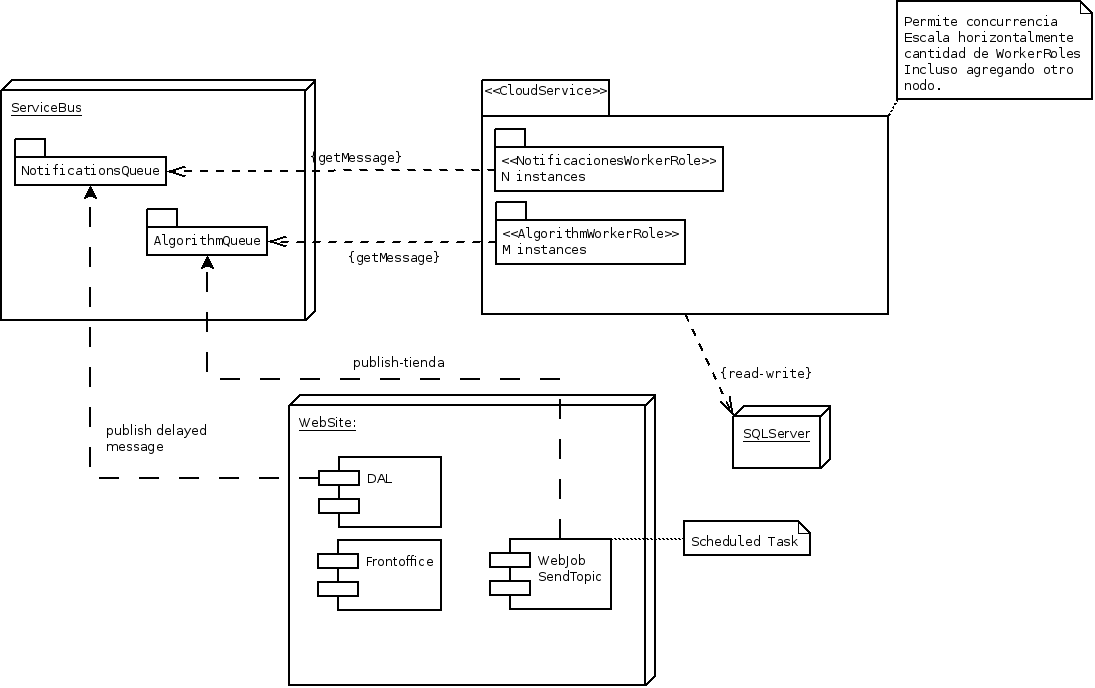
\includegraphics[width=3in]{./figuras/despliegue.png}
  \caption{Diagrama Despliegue}
  \label{fig:despliegue}
\end{figure} 


\subsubsection{Ofertar Producto}
El usuario autenticado puede realizar una oferta tanto desde la página principal donde se ofrece un listado de productos, o desde la vista detallada del producto, accesible al hacer click en cualquiera de los productos listados de la página principal o por medio del buscador de productos.

Lo más interesante que se brinda en cuanto a esta funcionalidad es el uso de SignalR para actualizar las ofertas realizados por todos los usuarios conectados a una tienda en vivo, y el uso de timers en cada producto para indicar cuánto falta para que se cierre la subasta.
Debido a que se puede ofertar tanto de la página principal como desde la vista del producto, las ofertas se actualizan en ambas vistas.

Cabe destacar que como también utilizamos Redis, si un usuario está conectado en otro servidor, también visualizará las ofertas realizadas en el instante.

\section{Arquitectura}
Se ha decidido utilizar un estilo arquitectónico en capas no estricto, en el que las capas más altas utilizan servicios definidos en las capas más bajas.
A continuación se presenta un esquema UML de la arquitectura planteada.

\begin{figure}[!h]
  \centering
    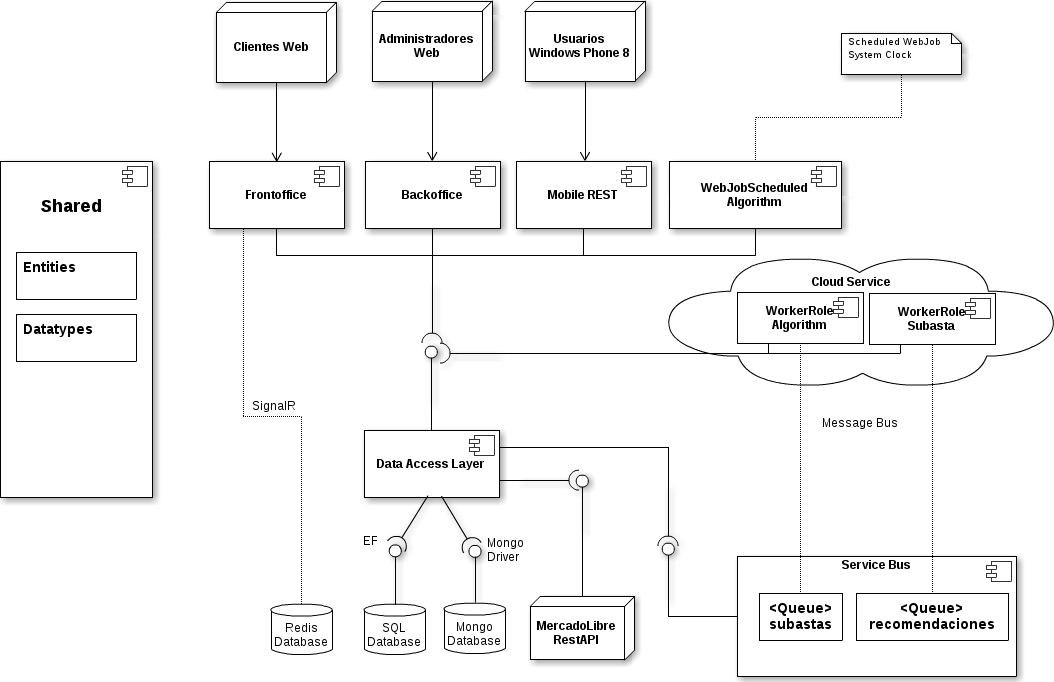
\includegraphics[width=3in]{./figuras/arquitectura.png}
  \caption{Arquitectura Sistema}
  \label{fig:arq}
\end{figure} 



\section{Implementación}

\subsection{Data Access Layer}
Esta capa implementa la funcionalidad de acceso a datos encapsulando la lógica para acceder a la base de datos. Provee interfaces para la capa lógica y la capa de presentación y accede a la base de datos. 
Se utilizó una estrategia intermedia para el manejo de datos entre distintos tenants. Por ello se seleccionó la estrategia separación por esquemas. Es decir un esquema por tienda. Brindando de esta forma un balance entre seguridad y escalabilidad del sistema. Resultó un enfoque complejo de implementar utilizando Entity Framework sin embargo se llegaron a buenos resultados en cuanto a la abstracción de cada tienda por esquema.\cite{url:schemadb}

\subsubsection{Productos y Herramientas}
Para realizar la capa de datos se definieron entidades y se utilizó Entity Framework como mapeador objeto-relacional para la creación de las tablas en SQL Server. Además, se utilizó la base de datos NOSQL MongoDB.
A continuación se realiza un análisis de las herramientas utilizadas: 
 

\begin{table}

\begin{center}
    \begin{tabular}{| p{1.5cm} | p{1.8cm} | p{1.8cm} | p{1.8cm} |}
    \hline
    \textbf{Producto} & \textbf{Puntos Fuertes)} & \textbf{Puntos Débiles} & \textbf{Evaluación General} \\ \hline
    Entity Framework &
    Facilidad de uso. &
    Documentación escasa con linq expressions. &
    Muy bueno.  \\ \hline
    
    SQL Server & 
    Servicio en Azure. Fácil administración. Integración con VisualStudio. & 
    &
    De gran utilidad integrando con Entity Framework. Con disponibilidad en Azure, se logró tener un único punto de acceso para testing. \\ \hline
    
    MongoDB &
    Flexibilidad $esquema$. Facilidad de uso y configuración. Disponibilidad. Escalabilidad horizontal. Replicación. &
    Aplicable a contextos que no requieran consistencia de datos. &
    De gran utilidad en el momento de generar las recomendaciones de productos para los usuarios. \\ \hline
    
    
    \end{tabular}
\end{center}
    \caption{Evaluación de Productos y Herramientas (Data Access Layer)}
    \label{tabla:dal}
\end{table}

\paragraph{MongoDB}
Basado en las características anteriores, se ajusta perfectamente a las necesidades del sistema. La finalidad del uso particularmente de un modelo no relacional tiene ventajas cuando el modelo de dominio puede compactarse en un único documento. Por ello esta tecnología se utilizó para la implementación del requerimiento relativo a la recomendación de productos.
Dicho requerimiento tiene características que permiten el uso de este modelo. Para cada usuario se obtiene un conjunto de productos, esto se puede compactar en un documento con llave primaria el usuario y los productos a ser listados.
¿Por qué utilizar Mongodb y no SQLServer para este requerimiento?
La respuesta tiene diversas aristas, en primer lugar las recomendaciones se realizan para todos los usuarios autenticados al sistema en la página principal. Si utilizamos como métrica la cantidad de consultas a la base que se debe realizar únicamente para este requerimiento secundario, posiblemente la performance del sistema se degrade en tiempos de respuesta. Entonces se independiza en un cluster mongo dicho requerimiento brindando además alta disponibilidad para el servicio, así como también la posibilidad de escalar horizontalmente si el contexto lo requiere.
La segunda arista consiste en la no estructuración de los datos. Supongamos una modificación en el esquema utilizado para las recomendaciones, utilizando un modelo relacional implica la tarea extra de alterar el esquema para que se adapte a las nuevas necesidades. En cambio con un esquema flexible los cambios no impactan directamente. Basta tomar la entidad o el datatype a persistir y adjuntarlo como un atributo de documento en formato json. Por tanto en la base pueden convivir distintos esquemas sin la necesidad de realizar la tarea de actualizarlos.
La tercer arista está relacionada con los mecanismos de alta disponibilidad que brinda Mongodb. Realizar replication es una tarea sencilla, además se puede distribuir el contenido de la base en distintas instancias mongod. Esta técnica se conoce como Sharding.

\paragraph{MongoDB Práctica}
Problemática análoga a la tecnología Redis, al ser privados de la licencia en Azure existieron limitaciones para los requerimientos los cuales utilizan esta tecnología. La solución es análoga al caso anterior, creación de una base en lal nube en el servicio MongoLabs. La versión gratuita básicamente provee las características necesarias para llevar a cabo la tarea. En la entrega final del producto existirá una instancia de Mongo, pero como brinda capacidad de escalabilidad horizontal de forma sencilla, la arquitectura permite el agregado de más instancias sin problemas mayores. El problema se remonta a obtener servidores que permitan mantener instancias de este tipo de bases.
Facilidad de uso, sintaxis sencilla, drivers completos para la mayoría de los lenguajes de programación. Al tratarse de un paradigma un tanto distinto al relacional, el concepto de colecciones es práctico, flexible y escalable. Las bases de datos pueden ser compartidas, así como en especial las colecciones, brindando versatilidad.

\subsubsection{Problemas Encontrados}
Los problemas consistieron en el momento de realizar modificaciones a nivel de esquema de la base. Debido a la complejidad del modelo separación por esquemas, cada vez que se creaba un tenant, se debía eliminar por completo el esquema anteriormente creado.


\subsection{Business Logic Layer}
\subsubsection{Productos y Herramientas}
La capa lógica implementa la funcionalidad principal de la aplicación Chebay. Encapsula la lógica de negocio relevante para la aplicación. Provee interfaces para la capa de Presentación y consume servicios de la capa de Datos. La principal funcionalidad que brinda es el sistema que cierra las subastas y envía notificaciones vía correo electrónico.

\subsubsection{Problemas Encontrados}
No existe una documentación actualizada sobre el Driver versión 2.0, sin embargo intuitivamente se puede lograr el cometido estudiando las clases brindadas en el NuGet.

\subsection{Presentation Layer}
La capa de presentación es la encargada de generar una interfaz web al usuario a través de un navegador web. Para esto genera una página consumiendo los servicios de la capa de datos.

\subsubsection{Productos y Herramientas}
El sistema a construir debía ser un sistema altamente interactivo para lograr que el usuario se sienta atraído al mismo. A la vez debía ser sobrio para lograr que el usuario permanezca la mayor cantidad de tiempo posible. Además, el sistema debía de escalar horizontalmente fácilmente, por lo que se decidió utilizar tecnologías que corrieran del lado del cliente, como JavaScript y jQuery para lograr alto grado de interactividad, evitar que el usuario tenga que esperar al realizar full requests y evitar cargar innecesariamente al servidor dejando parte de la lógica del lado del cliente. Todas las solicitudes, tanto de pedidos como de envío de formularios, se realizaron a través de AJAX. Para el diseño de la página web se utilizó html5/css3, se realizaron dos templates diferentes para personalizar la tienda, y ambos son responsive en su página principal, esto se logró con el uso de media querys. Además se utilizaron librerías como Boostrap y FontAwesome para utilizar componentes ya diseñados, y Animate.css para utilizar animaciones css3 y mejorar la experiencia del usuario.
Otra librería interesante que se utilizó es MustacheJS, básicamente permite definir templates mustache con tags (los tags hacen referencia a una clave), a este template se le inyecta un objeto javascript y el resultado es un código HTML en el cual los tags definidos previamente fueron sustituidos por los valores del objeto javascript. Esto es muy útil para renderizar información de manera simple cuando se obtiene el resultado de una llamada Ajax.

Se utilizó SignalR (librería para .NET que implementa Socket.io) y Redis para comunicar a todos los nodos de Windows Azure en donde se ejecuta la aplicación de forma simple y escalable.

A continuación se presenta un análisis de las tecnologías utilizadas en la capa de presentación. 


\begin{table}

\begin{center}
    \begin{tabular}{| p{1.5cm} | p{2cm} | p{2cm} | p{1.5cm} |}
    \hline
    \textbf{Producto} & 
    \textbf{Puntos Fuertes)} & 
    \textbf{Puntos Débiles} & 
    \textbf{Evaluación General} \\ \hline
    
    MomentJS &
    Simplifica el manejo de los timers. Fácil uso. Cumple con su cometido. &
    No tiene. &
    Excelente  \\ \hline
    
    Mustache JS & 
    Permite definir templates reutilizables. Mejor organización del código html. Simplifica el despliegue de los datos de manera dinámica. &
    No tiene. &
    Excelente \\ \hline
    
    SweetAlert &
    Buen diseño. Fácil de usar. &
    Las alertas de tipo confirm de la librería no se bloquean a la espera de la respuesta del usuario como si lo hace windows.confirm. &
    Muy buena \\ \hline
    
    FontAwesome &
    Gran cantidad de iconos. &
    No tiene. &
    Muy buena \\ \hline
    
    Animate.css &
    Permite realizar animaciones css3. Fácil de usar. Mejora experiencia del usuario. &
    No tiene. &
    Excelente \\ \hline
    
    Bootstrap &
    Simplifica tareas de diseño. Gran cantidad de componentes resueltos. &
     &
    Muy buena \\ \hline
    
    JQuery &
    Excelente herramienta para manipular el DOM del documento y el envió peticiones AJAX. &
    No tiene. &
    Excelente \\ \hline
    
    WebSockets / SignalR &
    Instalación sencilla. Curva de aprendizaje baja. Escalabilidad horizontal. &
    No tiene. &
    De uso obligatorio. \\ \hline
    
    Redis &
    Base de datos rápida. Instalación online o local. Publish Subscribe Colas.&
    No tiene cola de mensajes demorados, para sustituir ServiceBus. &
    Excelente \\ \hline
    
    
    
    \end{tabular}
\end{center}
    \caption{Evaluación de Productos y Herramientas  (Presentation Layer)}
    \label{tabla:pres}
\end{table}

\paragraph{Redis}
Entre sus funcionalidades se destaca la metodología publish-subscribe, permitiendo realizar replication. La existencia de colas de mensajes brinda la capacidad para establecer procesos asíncronos.
En el desarrollo del sistema se utiliza la funcionalidad Publish/Subscribe en combinación con Websockets para la implementación del chat, así como también la actualización en tiempo real de las ofertas sobre los productos.
La integración resultó sencilla, a lo que refiere órdenes de tiempo se logró implementar la infraestructura al cabo de un día. Primeramente se procedió a la creación de una máquina virtual linux en Windows Azure, se instaló Redis en la misma y se obtuvo la dirección de la vm para poder integrar en la configuración del Hub realizando un mapping hacia el servicio Redis.

\paragraph{Redis Práctica}
En primera instancia como se comentó anteriormente se utilizó una máquina virtual en la cual se procedió a la instalación del servicio Redis. No existieron problemas para llevar a cabo las operaciones de instalación.

La tarea que demandó mayor tiempo es la investigación de la tecnología, investigar la finalidad de la misma y en cuáles casos de uso sería conveniente utilizarla.
En segunda instancia se procedió a cambiar el servicio. El motivo principal es la cancelación de la suscripción a servicios de Azure, expiró la licencia brindada en el curso.
Como los tiempos apremian, se debió buscar una solución alternativa. La solución consistió en la creación de una cuenta en Redis Cloud, el cual brinda una base Redis con un límite de Storage de 30 MB. Considerando el método publish-subscribe la quota para lo que respecta el uso de Redis en el desarrollo del proyecto no presenta interés.
La migración para esta plataforma resultó ser más simple que la primera, en cuanto a la implementación se debió modificar únicamente una línea especificando la dirección del nuevo servidor. Un punto a favor de la arquitectura y la tecnología utilizada, probablemente si se utilizara una tecnología plenamente dependiente de la infraestructura Azure el cumplimiento de los requerimientos podría verse reducido en tiempo.

\paragraph{SignalR}
Los casos de uso Chat y visualización de ofertas en tiempo real, utilizan esta tecnología para brindar las funcionalidades tales como escalabilidad horizontal, visualización de ofertas en tiempo real. El primer hito parte de la base del uso de Redis como base de datos y la implementación de Websockets. En combinación se logra obtener un sistema escalable con la estrategia publish-subscribe. Logrando independizar en un servidor dedicado el servicio Redis, incrementando la performance y tiempo de respuesta del sistema.
La propuesta de SignalR consiste en implementaciones tanto del lado del cliente como del servidor. Del lado del servidor se publica un Hub, en el caso particular para desarrollo web se encarga de brindar una descripción en un archivo javascript para que el cliente pueda obtener la información de la conexión. La aplicación requiere implementación en javascript por el lado del cliente. La integración con Redis se realiza por la metodología Publish-Subscribe, mediante el uso del hub se crean $topics$, los clientes están suscriptos a los mismos y también realizan la función de publicar.
La escalabilidad se logra configurando el Hub con mapeo hacia el servicio Redis. La justificación se basa en escalar horizontalmente en número de servidores web, sin Redis esto no es posible puesto que los clientes obtendrán los mensajes únicamente del servidor en que se encuentren conectados. En cambio con Redis se logra eliminar dicho obstáculo, todos los hubs utilizan el mismo servicio por tanto clientes conectados en servidores web distintos pueden estar suscritos al mismo $topic$.

\paragraph{SignalR Práctica}
La principal dificultad radica en informarse cómo utilizar la tecnología en los casos de uso que así lo requerían. En el proyecto Chebay.Frontoffice se crearon dos hubs para la tarea del chat, y las notificaciones de ofertas en tiempo real. En cuanto a tiempo refiere la implementación 20 minutos para escribir las clases correspondientes.
Del lado del cliente se utilizó javascript, al igual que en el lado del servidor el tiempo de implementación es reducido.
La tecnología está consolidada, existe gran volumen de documentación, además de brindar las características deseables para que el producto sea escalable.
No existieron problemas relacionados con esta tecnología, la curva de aprendizaje es reducida.

\subsubsection{Problemas Encontrados}
Deploy de algunos archivos javascript en Azure. Posteriormente se agrega el problema de la licencia debido al alto consumo de poder computacional por parte del equipo.

\section{Evaluación de la Solución}
En lo que respecta a los puntos \ref{sec:cierresubasta} y \ref{sec:recomendacionproductos} se logra el performance descrito en cuanto a consumo de CPU. En la imagen \ref{im:cloudservice} se destaca el consumo promedio ni siquiera alcanza el 2\% logrando un rendimiento óptimo en comparación a la primera implementación por medio del pooling.
Sin lugar a dudas la solución agregó complejidad a nivel arquitectónico, a cambio de rendimiento y desacoplamiento del sistema.


\begin{figure}[]
  \centering
    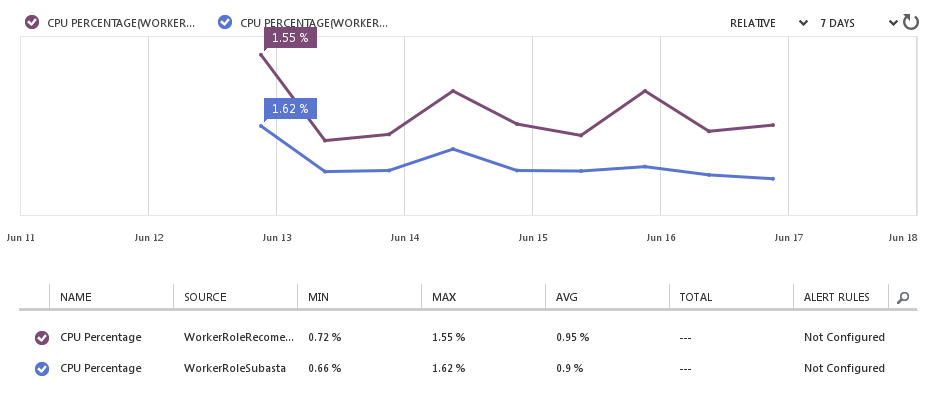
\includegraphics[width=3in]{./figuras/cloudservice.png}
  \caption{Performance Cloud Service + Service Bus}
  \label{im:cloudservice}
\end{figure} 

En general, se confía en haber realizado un buen diseño de la realidad teniendo en cuenta tanto los requerimientos funcionales como los no funcionales.

En relación al diseño visual de la aplicación, se logró realizar una interfaz altamente interactiva, en la que se realizan casi todas las consultas en segundo plano a través de AJAX ofreciendo una gran experiencia para el usuario. En nuestra opinión, esta es una característica muy importante de nuestra aplicación.

En cuanto al rendimiento, se intentó que gran parte de la lógica se encuentre del lado del cliente aumentando el rendimiento al reducir la cantidad de datos transmitidos a través de internet. Además, se logró reducir la carga al servidor, permitiendo un mejor aprovechamiento de los recursos. La capa de presentación envía y recibe los datos directamente de la capa de acceso a datos, evitando pasar por la capa de negocios, aumentando el rendimiento del sistema.

Se prestó especial atención a que el sistema pueda escalar horizontalmente de forma fácil en Windows Azure... 

\section{Desarrollo del Proyecto}
En esta sección se describe como fue el desarrollo de la plataforma. Primero se describirán las etapas del proyecto, luego se atacará el cronograma y por último se realizará un análisis del desarrollo.

\subsection{Etapas del Proyecto}
El proyecto se descompuso en cuatro etapas:

\subsubsection{Investigación}
En esta primera etapa, los integrantes del grupo investigaron las funcionalidades de la plataforma .NET y las prestaciones brindadas por Microsoft Azure. Se hizo una evaluación y selección de tecnologías a utilizar como SignalR, EntityFramework y varias librerías JavaScript para la parte web. Esta tarea fue realizada de forma individual por cada integrante excepto la parte de evaluación y selección de tecnologías, la cual fue grupal.

\subsubsection{Diseño y prototipado}
Esta etapa fue de alta importancia en el desarrollo del proyecto ya que se pudo definir la arquitectura del sistema. Cabe destacar que se cambió bastante la arquitectura a lo largo del proyecto principalmente por ser el primer acercamiento a este tipo de tecnologías. El diseño del prototipo permitió definir una arquitectura más sólida e implementar gran parte de los requerimientos funcionales pudiendo estimar cuál sería el alcance de nuestra solución final y aproximar el tiempo requerido para desarrollar ciertas funcionalidades.

\subsubsection{Desarrollo del sistema}
En esta etapa se completó la totalidad del desarrollo del sistema completando el alcance propuesto.

\subsubsection{Documentación}
Por último, se escribió la documentación final, la cual este artículo es una parte importante.


\subsection{Metodología}
La metodología de trabajo fue constante durante todo el desarrollo del proyecto. Consistió en las siguientes actividades.

Se realizaron reuniones semanales de aproximadamente dos horas, en las que cada integrante comentaba y mostraba el trabajo realizado en esa semana. Además, se discutían los problemas encontrados, analizando soluciones y alternativas para los mismos. Por último, se planificaba el trabajo para la semana siguiente, realizando una separación de tareas para cada integrante de forma que se sabía quién era el responsable de cada parte del proyecto. Se utilizó la herramienta de gestión de proyectos Teamwork \cite{url:teamwork}, para coordinar el trabajo grupal, asignar tareas, describir las mismas, discutir problemáticas y posibles soluciones.

Cada integrante trabajaba diariamente en las actividades planificadas en la reunión semanal de forma individual comunicándose con el resto de los integrantes mediante correo electrónico y un grupo de Whatsapp.

\subsection{Cronograma}

\subsection{Análisis del Proyecto}

\section{Conclusiones y trabajo a futuro}
En general, confiamos en haber realizado un proyecto exitoso habiendo cumplido con todos los requerimientos tanto funcionales como no funcionales además de haber implementado varios opcionales.

Fue altamente efectivo el uso de tecnologías como JavaScript que se ejecutan en el navegador del cliente para lograr una experiencia muy dinámica y satisfactoria. Además, fue muy positivo el uso de SignalR que permitió implementar varias funcionalidades de tiempo real de forma muy efectiva y atractiva para el usuario final.

Como un primer acercamiento a trabajar con tecnologías en la nube de Windows Azure, se concluye que existe un enorme potencial de esta tecnología. Permite una gran flexibilidad y una posibilidad de tener una plataforma con una enorme capacidad sin las complicaciones de configuración e instalación. Como crítica, para un proyecto en desarrollo como el nuestro que no ha sido liberado en producción, se gastaron más de 200 dólares en aproximadamente dos meses, por lo que al aumentar el número de usuarios esta tecnología puede ser bastante cara.

En relación al trabajo futuro, se puede expandir la solución para aumentar el nivel de escalabilidad del sistema. Se describe a continuación algunos puntos importantes que se pueden lograr en trabajos futuros.

\begin{itemize}
  \item Alta disponibilidad MongoDB: En el proyecto final se utilizó una instancia Mongo, no solventa el problema de eventuales fallos. Se puede implementar estrategias de particionado en las colecciones, agregado de replica-sets para generar una estrategia de HA\&DR (High Availability \& Disaster Recovery). Incrementando de esta forma la performance tanto en lectura como escritura, con el uso de un cluster mongodb.
  \item Algoritmo de Recomendación: Realizar un estudio detallado sobre las diferentes opciones disponibles para mejorar el nivel de seguridad para la estrategia .dll. Esto se puede llevar a cabo con la restricción de la utilización de namespaces, una tarea compleja de ser llevado a cabo. Otra alternativa es el uso de lenguajes interpretados como ser Python, Ruby, Perl, entre otros. Mantener la estrategia de Worker Role pero para otra plataforma y lenguaje, utilizando un sistema operativo Linux para la ejecución del mismo. Se puede lograr incluso mejoras sustanciales utilizando crontab para establecer los horarios oportunos para la ejecución.
  \item Sistema de alertas subasta/compra producto: Crear notificaciones adicionales sobre acontecimientos en la tienda. Integración con Twitter, generar heurísticas que utilice hashtag para definir tendencias de los productos de la tienda y de esta forma generar una notificación a todos los usuarios recomendando el producto. Mejorar a la vez el sistema de calificación de usuario, esto es programando un horario posterior a la adquisición del producto alentando al usuario a calificar al vendedor.
  \item Login: Proceso de autenticación utilizando cuentas en diversas redes sociales (Gmail, Twitter, LinkedIn, etc).
  \item Implementar el inicio de sesión en la aplicación de Windows Phone. 
  \item Agregar seguridad a la API REST.
\end{itemize}


\bibliographystyle{IEEEtran}%{unsrt}
\bibliography{bibliografia}


\end{document}
